\documentclass[10pt]{article}

\usepackage{graphicx}
\usepackage{amsmath}
\usepackage[T1]{fontenc}
\usepackage[utf8]{inputenc}
\usepackage[spanish]{babel}
\usepackage{babelbib}
\usepackage{color}
\usepackage{framed}
\usepackage{hyperref}
\usepackage{listings}


\definecolor{red}{RGB}{219,0,0}
\definecolor{pink}{RGB}{255,100,100}
\definecolor{gray}{RGB}{100,100,100}
\lstset{
		basicstyle=\ttfamily,
		frame=single,
		keywordstyle=\color{red},
		commentstyle=\color{gray},
		stringstyle=\color{pink},
		tabsize=3,
		language=verilog,
		backgroundcolor=\color{white}}

\usepackage{fancyhdr} 
\pagestyle{fancy}
\usepackage{lastpage}
\lhead{Laboratorio 2}
\chead{}
\rhead{Anteproyecto}
\lfoot{}
\cfoot{}
\rfoot{\footnotesize Page \thepage\ of \pageref{LastPage}}

\renewcommand{\headrulewidth}{0.4pt} 
\renewcommand{\footrulewidth}{0.4pt} 

\graphicspath{{../media/}}	%%multimedia path
\setlength{\parindent}{0pt}
%%*************************************************************************
\begin{document}

\begin{huge}
\begin{center}
\textbf{Anteproyecto 4: VGA}
\end{center}
\end{huge}

\begin{Large}
\begin{center}
Jose Apú (B10407), Francisco Molina (B12345), \\Marco Montero (A94000), Dennis Vargas (B16831)
\end{center}
\end{Large}

\section*{Objetivo General}
Utilizar los periféricos de la tarjeta de desarrollo.

\section*{Objetivos específicos}
\begin{itemize}
\item Investigar cómo utilizar periféricos en la tarjeta de desarrollo.
\item Realizar interfaz entre el usuario y Spartan 3E Starter kit.
\item Realizar interfaz entre el usuario y Papillio Duo.

\end{itemize}

\newpage

\section*{Ejercicio1}
\subsection*{Solución Propuesta}
Para este proyecto se utilizará la tarjeta Papilio Duo en lugar de la Spartan 3E, esta posee un shield con una entrada VGA.
Para el control de la entrada VGA, con cada flanco de reloj se lee la memoria de video que corresponde al color de una fila y columna específica.
Conforme se va escribiendo en cada columna, se utiliza una señal de sincronización vertical para escribir el dato en el pixel correspondiente o deseado. Cuando se termina una de las filas de la pantalla, se utiliza una señal de sincronización horizontal para pasar a la siguiente fila de la pantalla. Una metáfora comparativa de este sistema sería una máquina de escribir que tiene un "sincronizador vertical" que alinea la letra a la columna y un "sincronizador horizontal" que al finalizar la fila, tira el tambor con la hoja a la primera posición de la siguiente fila.
Se necesitará entonces crear un módulo controlador VGA que se encargará de controlar las señales de sincronización y los colores que se asignaran a los pixeles. El controlador seguirá las siguientes especificaciones temporales.
\begin{center}
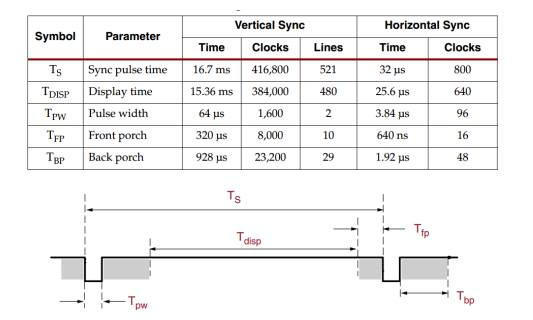
\includegraphics[width= 10cm]{sinc.jpg}
\end{center}
Un código viable para el módulo es el siguiente:
\begin{lstlisting}
module VGA_controller
(
input wire pixel_Clock , // 50 MHz
input wire pixe l_reset,
input wire pre_reset ,
output reg oVGA_HSYNC,
output reg oVGA_VSYNC,
output wire [2:0] oVGA_RGB
);

wire [9:0] wHorizontal_counter ;
wire [9:0] wVer t ical_counter ;
assign oVGA_RGB = {1'b1 ,1'b0,1'b0} ;
reg fila_final,columna_final ;

// contador es de filas y columnas
UPCOUNTER_POSEDGE #(10) contador_columnas (
.Clock (pixel_Clock),
.Reset (pixel_reset|columna_final), // 
.Initial(10'b0),
.Enable(1'b1),
.Q(wHorizontal_counter)
);

UPCOUNTER_POSEDGE#(10)contador_filas( 
.Clock(pixel_Clock), 
.Reset(pixel_reset|fila_final), 
.Initial(10'b0), 
.Enable(columna_final), 
.Q(wVertical_counter) 
);

always@(posedge pixel_Clock ) 
if(pixel_reset) 
begin 
columna_final <= 1'b0; 
fila_final <= 1'b0; 
oVGA_VSYNC = 1'b1; 
oVGA_HSYNC = 1'b1; 
end
else 
begin 
// oVGA_RGB <= {1'b1,1'b0,1'b0}; 
// columnas 
if(wHorizontal_counter == 10'd399 ) 
// ultima columna 640+160 10'd799
begin
columna_final <= 1'b1;
oVGA_HSYNC = 1'b1;
end
else if( wHorizontal_counter > 10'd326 
&& wHorizontal_counter < 10'd372) //655 
begin
columna_final <= 1'b0;
oVGA_HSYNC = 1'b0;
end
else
begin
columna_final <= 1'b0;
oVGA_HSYNC = 1'b1;
end
//filas
if(wVertical_counter == 10'd259) //521
begin
fila_final <= 1'b1;
oVGA_VSYNC = 1'b1;
end
else if( wVertical_counter > 10'd245 
&& wVertical_counter < 10'd247) //490 & 492
begin
fila_final <= 1'b0;
oVGA_VSYNC = 1'b0;
end
else
begin
fila_final <= 1'b0;
oVGA_VSYNC = 1'b1;
end
end
endmodule

\end{lstlisting}

 Además se debe crear un módulo de memoria RAM(de video) aparte del módulo RAM ya existente. Esto porque la memoria RAM de video se encargará de guardar los bits correspondientes a los colores de los pixeles que se van a desplegar en pantalla.La resolución que se decidió utilizar es 256x256 pixeles ya que la SPARTAN no tiene suficiente capacidad para soportar toda la resolución de una pantalla como las del laboratorio. 

\section*{Ejercicio 2}
\subsection*{Solución Propuesta}
Para este segundo ejercicio como no se utilizará la SPARTAN 3E la entrada de datos no se hará por medio de un teclado sino a través de una pequeña interfaz que posee el shield, que tiene 4 botónes, arriba,abajo,derecha e izquierda.
De no existir uno, se deberá crear una controlador para la botonera, el cual lo que hará es leer cuando uno de los botones se presiona.
Luego con la ayuda de la memoria de video se creará un tablero de ajedrez y se guardará la posición del cuadro inicial, además una máquina de estados se encargará de ver en cual cuadro se encuentra y cual de los botonés se precionó para moverse al próximo cuadro. A la salida de la memoria de video se verificará si se van a mostrar los datos del cuadro al que se quiere ir, si se comprueban entonces el cuadro se pinta de color rojo.
\end{document}
%%*************************************************************************
